\documentclass[a4paper,12pt]{report}

\usepackage{float}
\usepackage[utf8]{inputenc}
\usepackage[margin=1in]{geometry}
\usepackage{url}
\usepackage[backend=bibtex]{biblatex}
\usepackage{commath}
\usepackage{multicol}
\usepackage{graphicx}
\usepackage{pdfpages}

\title{CS699 Software Lab Project}
\author{Swarupananda Dhua(22M2102) and Akshat Gautam(190110004)}

\begin{document}

\maketitle

Project Idea: The name of the Game is “COVID Combat”. It’ll be a game running in 2D. There will be a battlefield consisting of empty places and obstacles through which the active objects of the game can walk and interact. The Player of the Game will have an unlimited supply of bullets using which he’ll kill the Coronaviruses. On the other hand, Coronaviruses will walk randomly and if the Player comes in contact, the game will be over. If all the Coronaviruses are killed, Player will win the game.

If time permits, we’ll make the 2D game look like 3D using Raycasting. We’ll also add some other passive objects such ass buildings, sky, hills, trees to make the game look better.

Technologies:
Python and Pygame for coding the logic
Latex for creating user manual/documentation for the game
HTML/CSS for updating the status of the development.


\newpage
Progress as on 09/10/2022

Following picture is a screenshot of the game:
1.	Grid for the playground has been made.
2.	The Player and Coronaviruses have been added but their behaviours are not yet fully functional.
3.	Sound effects (for background music and player move) have been added.

Next steps: Collision detection between Player and Coronavirus, Shooting Bullets by the Player, Collision Detection between Bullet and Coronavirus.

\newpage
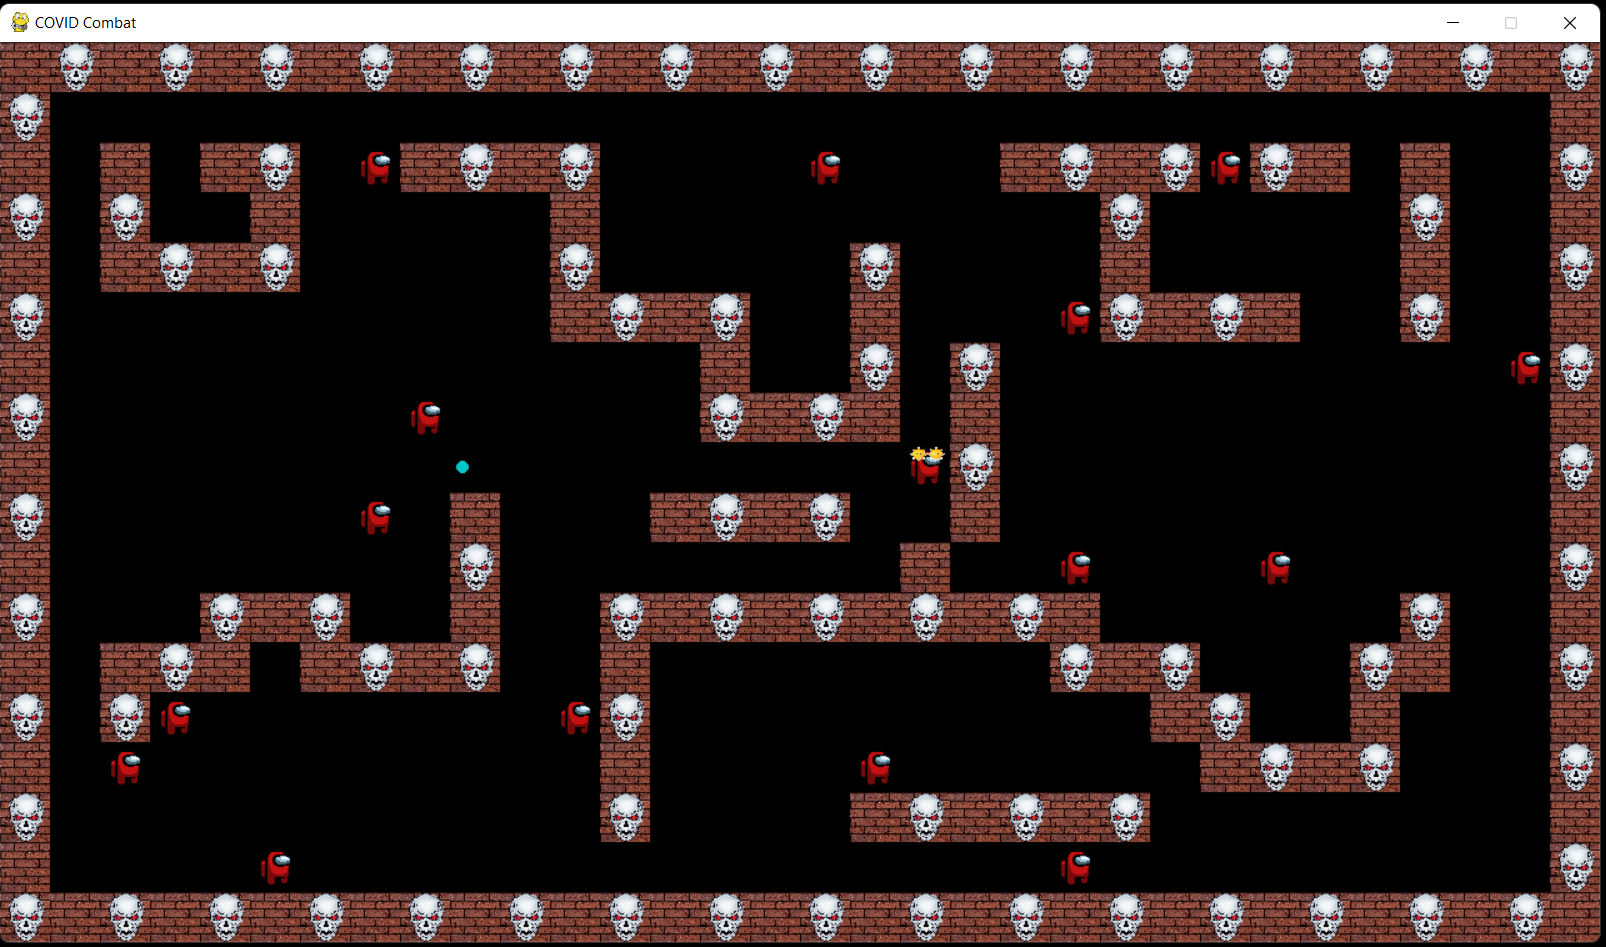
\includegraphics[scale=0.3]{snapshot.png}
\end{document}